%!TeX encoding = ISO-8859-1
\documentclass[12pt, a4paper, english]{tutthesis}

\usepackage{mathtools}
\usepackage{listings}
\usepackage{caption}
\usepackage{graphicx}
\graphicspath{ {images/} }
\usepackage{lmodern}
\usepackage{enumitem}

% Ensure the correct Pdf size (not needed in all environments)
\special{papersize=210mm,297mm}

% Define your basic information
\author{Jonne Petteri Pihlanen}
\title{Building a Recommendation Engine with Apache Spark}      % primary title (for front page)
\titleB{Suosittelijaj�rjestelm�n rakentaminen Apache Sparkilla} % translated title for abstract
\thesistype{Master of Science thesis} % or Bachelor of Science, Laboratory Report... 
\examiner{????} % without title Prof., Dr., MSc or such

% Special trick to use internal macros outside the cls file
% (e.g. \@author). Trick is reversed with \makeatother a bit later.
\makeatletter

% Define the pdf document properties.  Fill in your own keywords.
\hypersetup{   
  pdftitle={\@title},
  pdfauthor={\@author},
  pdfkeywords={recommmendation}
}

\usepackage[english]{babel}

\pagenumbering{Roman}
\pagestyle{headings}
\begin{document}

% Create the title page.
\thispagestyle{empty}
\vspace*{-1cm}\noindent

\includegraphics[width=8cm]{tty_tut_logo}

% Then lay out the author, title and type to the center of page.
\vspace{6.8cm}
\maketitle
\vspace{7cm} % modify if thesis title needs many lines

% Last some additional info to the bottom-right corner
\begin{flushright}  
  \begin{minipage}[c]{6.8cm}
    \begin{spacing}{1.0}
      \textsf{Examiner: \@examiner}\\
      \textsf{Examiner and topic approved by the}\\ 
      \textsf{Faculty Council of the Faculty of}\\
      \textsf{xxxx}\\
      \textsf{on 1st September 2014}\\
    \end{spacing}
  \end{minipage}
\end{flushright}

% Leave the backside of title page empty in twoside mode
\if@twoside
\clearpage
\fi

\pagenumbering{roman} 
\setcounter{page}{0} % Start numbering from zero because command 'chapter*' does page break


% Some fields in abstract are automated, namely those with \@ (author,
% title in the main language, thesis type, examiner).

% !!! Problems with other language. Disable it (ES, 2014-11-03)
%%\begin{otherlanguage}{english} %  Following text in in 2nd language
\chapter*{Abstract}

\begin{spacing}{1.0}
         {\bf \textsf{\MakeUppercase{\@author}}}: \@title\\   % use \@titleB when thesis is in Finnish
         \textsf{Tampere University of Technology}\\
         \textsf{\@thesistype, xx pages} \\
         \textsf{September 2016}\\
         \textsf{Master's Degree Program in Signal Processing}\\
         \textsf{Major: Data Engineering}\\
         \textsf{Examiner: \@examiner}\\
         \textsf{Keywords: }\\
\end{spacing}

The amount of recommendation engines around the Internet is constantly growing.

This paper studies the usage of Apache Spark when building a recommendation engine.

\chapter*{Tiivistelm�}

\begin{spacing}{1.0}
         {\bf \textsf{\MakeUppercase{\@author}}}: \@titleB\\  % or use \@title when thesis is in Finnish
         \textsf{Tampereen teknillinen yliopisto}\\
         \textsf{Diplomity�, xx sivua}\\ %
         \textsf{syyskuu 2016}\\
         \textsf{Signaalink�sittelyn koulutusohjelma}\\
         \textsf{P��aine: Data Engineering}\\
         \textsf{Tarkastajat: \@examiner}\\
         \textsf{Avainsanat: }\\
\end{spacing}

\makeatother % Make the @ a special symbol again, as \@author and \@title are not neded after this


\chapter*{Preface}

ASDASDASDASDASD


~ 
% Tilde ~ makes an non-breakable spce in LaTeX. Here it is used to get
% two consecutive paragraph breaks

Tampere, 

~


Jonne Pihlanen




%
% Add the table of contents, optionally also the lists of figures,
% tables and codes.
%

\renewcommand\contentsname{Table of Contents} % Set English name (otherwise bilingual babel might break this), 2014-09-01
%\renewcommand\contentsname{Sis�llys}         % Set Finnish name
\setcounter{tocdepth}{3}                      % How many header level are included
\tableofcontents                              % Create TOC

%\renewcommand\lstlistlistingname{List of Programs}      % Set English name (otherwise bilingual babel might break this)
%%\renewcommand\lstlistlistingname{Ohjelmaluettelo} % SetFinnish name, remove this if using English
%\lstlistoflistings                                % Optional: create the list of program codes
%\markboth{}{}                                     % no headers


%
% Term and symbol exaplanations use a special list type
%

\chapter*{List of abbreviations and symbols}
\markboth{}{}                                % no headers

% You don't have to align these with whitespaces, but it makes the
% .tex file more readable
\begin{termlist}
	\item [Recommendation Engine]	System that tries to predict the items that a user woud like
	\item [Collaborative]			Users collaborate with each other to recommend items
	\item [Spark] 					Fast and general engine for large-scale data processing
	\item [Information retrieval (IR)]	Activity of obtaining relevant information resources from a collection of information resources.
	\item [SDK] Software Development Kit
\end{termlist}

% Leave the backside of abbreviation list empty in twoside mode
\cleardoublepage

% The actual text begins here and page numbering changes to 1,2...
\newpage             % needed for page numbering
\pagenumbering{arabic}
\setcounter{page}{1} % Start numbering from zero because command
                     % 'chapter*' does page break
\renewcommand{\chaptername}{} % This disables the prefix 'Chapter' or
                              % 'Luku' in page headers (in 'twoside'
                              % mode)

\chapter{Introduction}

Recommender systems have been successfully utilized to aid customers in decision making.
In fact, they are constantly present in our everyday life.
Whether a customer is shopping online, watching a movie from Netflix, browsing the Facebook or simply reading the news.
All of these tasks involve a presence of a recommendation engine.
Basically all parts of our daily life include recommendations of some sorts.
However, the most basic type of recommendation is the one from human to human and happens completely without computers.

Recommendation can be divided into two major categories: item based and user based.

%Present state of recommendation is to incorporate context awareness into recommendation. Context and Context Aware Recommendation Systems (CARS) are described in Chapter 2.

This thesis is structured as follows.
Chapter 2 describes recommendation systems.
In Chapter 3, the data for this project and related tasks are discussed.
Chapter 4 discusses Apache Spark, an open source framework for building distributed programs.
Chapter 5 discusses the results. Finally, in Chapter 6 the evaluation is presented along with conclusions.

%Bigger companies have also released directly and indirectly their open source recommendation solutions. Twitter contributed to Spark project directly by releasing the DIMSUM algorithm, short for Dimension Independent Matrix Square using MapReduce, which limits the list of potential combinations to a reasonable number, enabling other recommendation algorithms to run in a reasonable amount of time \cite{harris14}. Netflix contributed indirectly by hosting the Netflix Prize competitions. Around these competitions, Alternating Least Squares (ALS) algorithm became popular and the ALS implementation in Spark MLlib is inspired by some of the solutions in the competition \cite{ryza15}. DIMSUM and ALS are described in chapter 5.

\chapter{Recommendation Systems}
\label{ch:rs}

Recommendation denotes a task in which items are recommended to users.
The most simple version of recommendation is from peer to peer, completely without computers.
However, humans can only recommend effectively those items they have personally experienced.
This is where recommendation systems (RSs) become useful as they can potentially offer recommendations from thousands of different items.
Recommender systems are a set of techniques and software tools that provide suggestions to users about potentially useful items.
Item denotes the general subject that the system recommends to users.
Recommendation systems are usually intended to recommend only specific kind of items such as books or movies. \cite{ricci11}

Recommendation systems are often targeted to aid customers in decision making when the amount of all items is overwhelming.
Usually the recommendations are personalized, which implies that the recommendations are different for different users or groups of users.
Recommendations can also be non-personalized and usually these are much simpler to generate.
A simple ranked top-ten list of items is an example of non-personalized recommendation.
Ranking is done by predicting the most suitable items based on the user's preferences and constraints.
To complete this task, RS needs to collect these preferences from users.
They might be explicitly expressed ratings for products or interpreted from user actions such as clicks and page viewsFor example, RS could consider navigation to a product page as an implicit evidence of preference for the items in that page\cite{ricci11}

Development of RSs initiated from a rather simple observation: people usually tend to trust recommendations provided by others in making routine decisions.
For example, it is common to rely on peer feedback when selecting a book to read or rely on the reviews the movie critics have writtenFirst RSs tried to mimic this behavior by applying algorithms to leverage recommendations from the community to an active user looking for recommendations. Recommendations were for users with similar tastes. This approach is essentially collaborative-filtering and the idea behind it is that if users liked similar items in the past, they are likely to consider recommendations from these same users relevant. \cite{ricci11}

Along with the development of e-commerce sites, a need for recommendations emerged to limit the amount of alternatives.
Users were finding it more and more difficult to find the correct choices from the vast range of items the sites were offering.
As the variety of information in the Web has explosively grown constantly overwhelmed users, it has led them to make poor decisions.
The availability of choices had begun to decrease users well-being, instead of producing benefit.
While choice is good, more choice is not always better. \cite{ricci11}

Recently, RSs have proved to be an effective cure for the information overload problem at hand.
RS addresses this phenomenon by offering new, previously unknown items that are likely to be relevant to the users current task.
When a user requests for recommendations, RSs generate recommendations by using knowledge and data about the users, available items and previous transactions present in the recommender database.
After browsing the provided recommendations, she may accept them or not thus providing implicit and explicit feedback to the recommender.
This new information can later on be used when generating new recommendations upon the next user-system interactions. \cite{ricci11}

Compared to research in the classical fields of information systems such as databases and search engines, study of recommender systems is relatively new.
They became an independent research area in the mid-1990s. Recently, the interest towards recommendation systems has dramatically increased.
Evidence can be found for example from such highly rated Internet sites as Amazon.com, YouTube, Netflix and IMDB in which RSs are playing an important role.
Another example are conferences and journal issues dedicated to RS research and development such as RecSys and AI Communications (2008), consecutively. \cite{ricci11}

Two primary purposes exist for a RS: first is to aid the service provider somehow and the other is to produce value to the user of the service.
Thus, a RS must balance between the needs of service provider and the customer \cite{ricci11}.
For example, a service provider might introduce a RS to get help in tasks such as increasing the number of items sold, selling more diverse items, increasing user satisfaction, increasing user loyalty or understanding better what the user wants \cite{ricci11}.
In addition, a number of different functions exist that the user might expect a recommendation system to offer. Some of these are similar to the ones mentioned above, thus considered as core functions.
For instance, a user may want a RS to recommend a sequence of items, aid in browsing or enable user to influence others users. Influencing might also be malicious. \cite{ricci11}

GroupLens, BookLens and MovieLens were pioneers in RSs.
Furthermore, they also released data sets which, aside of recommendation, was also pioneering in the field. Data sets were not that common for benchmarking or just trying out new technologies. \cite{aggarwal16}

% TODO: how to include this?
%A Recommendation engine system or part of it can also be acquired via a competition such as the Netflix prize competition held in 2007, 2008 and 2009. As a result, Netflix's algorithm was beaten by 10.05\%\ . Sequels were canceled due to privacy concerns. Two people were apparently able to reveal the identities of users by matching the rating data to those of Internet Movie Database (IMDB) thus finding out the identities of IMDB users. Netflix (Netflix Prize competition, winner used RBM) \cite{bell06} \cite{koren09}.

\section{Recommendation techniques}

Recommendation system must have some sort of understanding about the items to be able to recommend something.
To achieve its goal, the system must be able to predict the usefulness or at least compare the utility of some items and then decide the ones to recommend.
The prediction step of the recommender can be illustrated by, for example, a simple non-personalized, recommendation algorithm that recommends only the most popular movies.
The reasoning behind this approach is that when lacking more precise information about the user's preferences, a movie liked by others is probably also liked by a general user, at least more than a randomly selected movie.
Thus, the utility of these popular songs can be seen reasonably high for a generic user. \cite{ricci11}

The utility of the user $u$ for the item $i$ can be modeled as a real valued function $R(u,i)$ as is normally done in collaborative filtering by considering the ratings of items given by the users.
Thus, the fundamental task of the collaborative filtering recommender is to predict the value of $R$ over pairs of users and items to compute an estimation for the true function $R$.
Consequently, by computing this prediction for the user $u$ on a set of items, the system will recommend items with the largest predicted degree of utility.
The amount of predicted items is usually much smaller than the whole amount of items, thus the RS is filtering the items that are recommended to users. \cite{ricci11}

RSs vary in terms of the addressed domain, the knowledge used and especially how the recommendations are made, denoting the recommendation algorithm \cite{ricci11}.
This thesis will concentrate only on one class of recommendation techniques, collaborative filtering, since that is the one used in Apache Spark's MLlib.

Collaborative Filtering Recommendation Systems are based on the collaboration of users.
They aim at identifying patterns of user interests in order to make targeted recommendations \cite{aberger14}.
The original implementation of this approach recommends to the active user those items that other similar users in the sense of tastes have liked in the past \cite{ricci11}.
First a user provides ratings for items.
Next the method will find recommendations based on other users that have purchased similar items or based on items that are the most similar to the user's purchases.
Collaborative filtering can be divided into two sub categories which are item-based collaborative filtering and user-based collaborative filtering.
Collaborative filtering has been studied the most thus being the most popular and widely implemented technique in recommendation systems \cite{gorakala15} \cite{ricci11} \cite{burke02}.

Collaborative filtering analyzes relationships between users and interdependencies among products to identify new user-item associations. \cite{korenBellVolinsky09}
For example, deciding that two users may both like the same song because they play many other same songs is an example of collaborative filtering. \cite{ryza15}

Collaborative filtering algorithms suffer from the new user and new item problems \cite{gorakala15}.
This originates to the fact that the recommendation is based only on user's recommendations on items.
If user has not given any reviews, the algorithm is not able to produce any recommendations either.
Other issues of collaborative filtering algorithms are cold start and sparsity.
Cold start denotes that a relatively large amount of data is required in order to be able to provide accurate recommendations for a user.
Sparsity means that the number of items typically exceeds the number of users.
This makes the relations extremely sparse since most users have rated or purchased only a small subset of the total items. \cite{aberger14}

Amazon.com, the biggest Internet retailer in the United States, has previously been using item-to-item collaborative filtering method.
However, the current status of Amazon recommendation seems to be unknown to the public, which, in fact, is better for the business.
In their implementation the algorithm builds a table containing similar items by finding ones that users tend to purchase together.
The algorithm then finds items similar to each of the user's purchases and ratings, combines those items, and returns the most popular or correlated items. \cite{linden03}

The following sections describe user-based collaborative filtering and item-based collaborative filtering.

\subsection{Item-based collaborative filtering}

Item-based collaborative filtering (IBCF) starts by finding similar items from the user's purchases \cite{gorakala15}.
Next step is to model the preferences of a user to an item based on ratings of similar items by the same user \cite{ricci11}.
The following snippet presents the idea in IBCF for every new user.

\lstset{
	columns=flexible,
	frame=single,
	breaklines=true
}

\begin{lstlisting}[caption=Item-Based Collaborative Filtering algorithm \cite{gorakala15}]

  1. For each two items, measure how similar they are in terms of having received similar ratings by similar users

  2. For each item, identify the k-most similar items

  3. For each user, identify the items that are most similar to the user's purchases
  

\end{lstlisting}

\subsection{User-based collaborative filtering}

User-based collaborative filtering (UBCF) starts by finding the most similar users, rate items purchased by similar users, pick top rated items.
The similarity in taste of two users is calculated based on the similarity in the rating history of the users \cite{ricci11}.

The steps for every new user in user-based collaborative filtering are as follows:

\lstset{
	columns=flexible,
	frame=single,
	breaklines=true
}

\begin{lstlisting}[caption=User-Based Collaborative Filtering algorithm \cite{gorakala15}]

  1. Measure how similar each user is to the new one. Like IBCF, popular similarity measures are correlation and cosine.

  2. Identify the most similar users. The options are:
	  Take account of the top k users (k-nearest_neighbors)
	  Take account of the users whose similarity is above a defined threshold

  3. Rate the items purchased by the most similar users. The rating is the average rating among similar users and the approaches are:
	  Average rating
	  Weighted average rating, using the similarities as weights

  4. Pick the top-rated items.
\end{lstlisting}

\chapter{Apache Spark}

Apache Spark is an open source framework that combines an engine for distributing programs across clusters of machines with an elegant model for writing programs. \cite{ryza15}
Spark provides high-level APIs in Java, Scala, Python and R.

At a high level, every Spark application consists of a driver and one or more executors.
Driver is a program that runs the user's main function and executes various parallel operations on a cluster.
An executor is one machine in a cluster.

Spark can be introduced by describing its predecessor, MapReduce, and the advantages it offers.
MapReduce offered a simple model for writing programs that could execute in parallel across hundreds of machines.
MapReduce achieves nearly linear scalability as the data size increases. The execution time is maintained by adding more computers to handle the task.

Spark preserves MapReduce's linear scalability and fault tolerance while extending it in three important ways.
In MapReduce the intermediate results between the map and reduce tasks must be written into memory where as Spark is able to pass the results directly to the next step in the pipeline.
Spark also treats the developers better by offering a rich set of transformations which enables users to represent complex pipelines in a few lines of code. (EXAMPLE?)
Spark also introduces in-memory processing by introducing Resilient Distributed Dataset (RDD) abstraction which offers a way for developers to materialize any step in a processing pipeline and store it into memory. This means that future steps do not need to calculate the previous results again.
Previously this kind of feature has not been available within distributed processing engines. \cite{ryza15}

Spark programs can be written using Java, Scala, Python or R.
However, using Spark with Scala instead of Java, Python or R has a couple of advantages to it.
Performance overhead is reduced, since tasks such as transferring data across different layers or performing transformations for data may result in weaker performance.
Spark is written with Scala, which denotes that user has always access to latest and greatest features of the framework.
Spark philosophy is easier to understand when Spark is used with the language it was built with.
There is still one, maybe the biggest benefit of using Scala with Spark, and it is the developing experience that comes with the fact that user is using the same language for everything.
Importing data from database, data manipulation, shipping the code into clusters. \cite{ryza15}

Spark is shipped with a read eval print loop (REPL), which enables developers to test out things quickly in the console, without having to make the application self contained from the begin.
Usually when a application developed in REPL has matured enough, it is a good idea to move it into a compiled library (JAR).
This way it is possible to prevent code and results from disappearing.

\section{Resilient Distributed Dataset (RDD)}

A Resilient Distributed Dataset (RDD), is the main abstraction in Spark.
Essentially it is an immutable, partitioned collection of elements that can be distributed across multiple machines in a cluster. \cite{spark-rdd}

An important context to understand about RDDs is that they are lazy by nature.
When a new RDD is created, nothing is actually done, it means that spark knows where the data is when the time comes to do something with it.

RDD can be created in two ways: parallelizing an existing Scala collection in the driver program or referencing an external dataset in an external storage system, such as HDFS, HBase or any file system supported by Hadoop \cite{spark-programming-guide}.

RDDs can be persisted into memory, which allows programmer to reuse them efficiently across parallel operations.
RDDs are able to recover from node failures automatically, using Directed Acyclic Graph (DAG) engine.
DAG supports cyclic data flow.
Each Spark job creates a DAG of task stages to be performed on the cluster.
Compared to MapReduce, which creates a DAG with two predefined stages - Map and Reduce, DAGs created by Spark can contain any number of stages.
This allows some jobs to complete faster than they would in MapReduce, with simpler jobs completing after just one stage, and more complex tasks completing a single run of many stages, rather than having to be split into multiple jobs. \cite{mapRSpark}

\begin{figure}[h]
	\caption{Directed Acyclic Graph \cite{dag-image}}
	\centering
	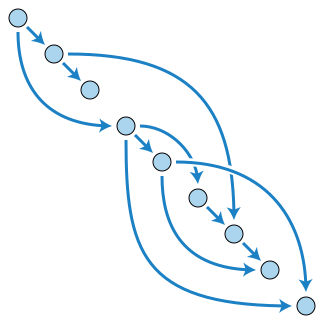
\includegraphics[scale=1.0]{directed_acyclic_graph}
\end{figure}

\section{Dataset API}

Dataset, DS, is the replacement for RDD in Spark.
It is a strongly typed collection of domain-specific objects that can be transformed in parallel using functional or relational operations.
Operations available on Datasets are divided into transformations and actions.
Transformations are operations such as map, filter, select and aggregate that produce new Datasets.
Actions are operations such as count, show, or writing data out to file systems that trigger computation and return results. \cite{spark-dataset}

Datasets are lazy by nature, which refers to that computations are only triggered when an action is invoked.
A Dataset essentially represents a logical plan that describes the computation required to produce the data.
Upon an action invocation, the query optimizer of Spark optimizes the logical plan and generates a physical plan for efficient execution in a parallel and distributed manner.
The logical plan as well as the optimized physical plan can be explored by using the explain function. \cite{spark-dataset}

To efficiently support domain-specific objects, an Encoder is required.
The encoder maps the domain specific type T to Spark's internal type system.
For example, given a class Person with two fields, name (string) and age (int), an encoder is used to tell Spark to generate code at runtime to serialize the Person object into a binary structure.
This binary structure often has much lower memory footprint as well as are optimized for efficiency in data processing (e.g. in a columnar format).
To understand the internal binary representation for data, use the schema function.

Two ways typically exist to create a Dataset.
The most common way is to make use of the read function provided by SparkSession and point Spark to some files on storage systems:

\lstset{
	frame=0,
	language=Scala
}

\begin{lstlisting}[caption=Creating a new Dataset by using read function]

val people = spark.read.json("./people.json").as[Person]

\end{lstlisting}

where $Person$ would be a Scala case class, for example:

\begin{lstlisting}[caption=Definition of case class Person]

case class Person(id: BigInt, firstName: String, lastName: String)

\end{lstlisting}

Case classes are normal Scala classes that are:

\begin{itemize}
	\item Immutable by default
	\item Decomposable through pattern matching
	\item Compared by structural equality instead of by reference
	\item Succinct to instantiate and operate on
\end{itemize}

If we would omit the casting with keyword $as$ then we would end up creating a DataFrame and the schema of the created object would be guessed by Spark.

SparkSession is the entry point to programming Spark with the Dataset and DataFrame API.
Datasets can also be created through transformations available on existing Datasets:

\begin{lstlisting}[caption=Creating a new Dataset through a transformation]

val names = people.map(_.name)

\end{lstlisting}

\cite{spark-dataset}

Datasets are similar to RDDs as they also provide strong typing and the ability to use powerful lambda functions \cite{spark-sql-programming-guide}. These are accompanied with the benefits of Spark SQL's optimized execution engine \cite{spark-sql-programming-guide}. However, instead of using standard serialization like Java serialization they use a specialized Encoder to serialize the objects.
Serialization denotes a task in which an object is turned into bytes thus reducing the memory footprint of the object.
In general, serialization is needed for processing or transmitting over the network.
While both encoders and standard serialization are responsible for turning an object into bytes, encoders are generated dynamically by code. They are using a format that allows Spark to perform many operations such as filtering, sorting and hashing without the need of deserializing the bytes back into an object. \cite{spark-programming-guide}

\section{DataFrame API}

Picture about rdd vs dataset vs dataframe ?

A DataFrame is essentially a Dataset that is organized into named columns.
In Scala, a DataFrame is represented by a Dataset of Rows.
It is conceptually equivalent to a table in a relational database or a data frame in R/Python, but it has richer optimizations under the hood.
DataFrames can be constructed from a range of sources such as structured data files, tables in Hive, external databases, or existing RDDs.
\cite{spark-sql-programming-guide}

\begin{figure}[h]
	\caption{DataFrame}
	\centering
	
\includegraphics[scale=1.0]{dataframe}
\end{figure}

\section{Matrix Factorization}

Matrix factorization denotes a task in which a matrix is decomposed into a product of matrices.
There are many different matrix decompositions.
The following chapter will describe matrix factorization in general and the Alternating Least Squares algorithm which is the matrix factorization algorithm that is implemented in Spark.
It is based on same idea as Netflix prize winner, matrix factorization models.

Matrix factorization belongs to a vast class of algorithms called latent-factor models.
Latent-factor models try to explain observed interactions between a large number of users and products through a relatively small number of unobserved, underlying reasons.
For example, they can try to explain why people would buy a particular album out of endless possibilities by describing users and albums in terms of tastes which are not directly available as data. \cite{ryza15}
A latent factor is not available for direct observation. For example health of a human being is a latent factor.
Health can not be observed as a variable such as blood pressure.

\begin{figure}[h]
	\caption{Matrix factorization \cite{ryza15}}
	\centering
	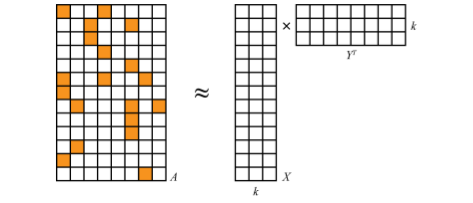
\includegraphics[scale=0.8]{matrix_factorization}
\end{figure}

Matrix factorization algorithms treat the user and product data as if it was a large matrix A.
Each entry in row $i$ and column $j$ represents a rating the user has given to a specific product. \cite{ryza15}

Usually $A$ is sparse, which denotes that most of the entries of $A$ are 0.
This is due to the fact that usually only a few of all the possible user-product combinations exist.

Matrix factorization models factor $A$ as the matrix product of two smaller matrices, $X$ and $Y$, which are quite tiny.
Since $A$ has many rows and columns, both of them have many rows, but both have just a few columns $(k)$. The $k$ columns match to the latent factors that are being used to explain the interactions of the data.
The factorization can only be approximate because $k$ is small. \cite{ryza15}

The standard approach to matrix factorization based collaborative filtering treats the entries in the user-product matrix as explicit preferences given by the user to the product, for example users giving ratings to movies.
Implicit data denotes for example page views or a value representing if a user has listened to a artist. Explicit data means actual ratings that a user has given to a product.
Spark ALS can handle both implicit and explicit data. \cite{spark14} \cite{ryza15}

Usually many real-world use cases have access only to implicit feedback data such as views, clicks, purchases, likes or shares.
However, instead of trying to model the matrix of ratings directly, the approach in Spark MLlib treats the data as numbers representing the strength of the observations such as the number of clicks, or the cumulative duration someone spent viewing a movie.
Instead of explicit ratings, these numbers are related to the level of confidence in observed user preferences.
Based on this data, the model tries to find latent factors that can be used to predict the expected preference of a user for an item. \cite{spark14}

Sometimes these algorithms are referred to as matrix completion algorithms.
This is because the original matrix $A$ may be sparse while the product $XY^T$ is dense.
Hence, the product is only an approximation of $A$. \cite{ryza15}
\subsection{Alternatig Least Squares (ALS)}

Collaborative filtering is commonly used for recommender systems.
These techniques aim to fill in the missing entries of a user-item association matrix.
Spark MLlib currently supports model-based collaborative filtering, in which users and products are described by a small set of latent factors that can be used to predict missing entries.
Spark MLlib uses the Alternating Least Squares (ALS) algorithm to learn these latent factors. \cite{spark14}

Spark ALS attempts to estimate the ratings matrix A as the product of two lower-rank matrices, $X$ and $Y$. \cite{als14}

\begin{equation}
A = XY^T
\end{equation}

Typically these approximations are refered to as factor matrices.
The general approach is iterative.
During each iteration, one of the factor matrices is held constant, while the other is solved for using least squares. The newly-solved factor matrix is then held constant while solving for the other factor matrix. \cite{als14}
Spark ALS enables massive parallelization since it can be done separately, it can be done in parallel which is an excellent feature for a large-scale computation algorithm. \cite{ryza15}

Spark ALS is a blocked implementation of the ALS factorization algorithm.
Idea is to group the two sets of factors, referred to as $users$ and $products$, into blocks.
Grouping is followed by reducing communication by only sending one copy of each user vector to each product block on each iteration.
Only those user feature vectors are sent that are needed by the the product blocks.
Reduced communication is achieved by precomputing some information about the ratings matrix to determine the out-links of each user and in-links of each product.
Out-link denotes those blocks of products that the user will contribute to.
In-link refers to the feature vectors that each product receives from each user block they depend on.
This allows to send only an array of feature vectors between each user block and product block.
Consequently the product block will find the users' ratings and update the products based on these messages. \cite{als14}

Essentially, instead of finding the low-rank approximations to the rating matrix $A$, it finds the approximations for a preference matrix $P$ where the elements of $P$ are $1$ when $r > 0$ and $0$ when $r <= 0$.
The ratings then act as confidence values related to strength of indicated user preferences rather than explicit ratings given to items. \cite{als14}

\begin{equation}
A_iY(Y^T Y)^{-1} = X_i
\end{equation}

Alternating Least Squares operates by rotating between fixing one of the unknowns $u_i$ or $v_j$.
While the other is fixed the other can be computed by solving the least-squares problem.
This approach is useful because it turns the previous non-convex problem into a quadratic that can be solved optimally \cite{aberger14}.
A general description of the algorithm for ALS for collaborative filtering taken from \cite{aberger14} is as follows:

\begin{lstlisting}[caption=Alternating Least Squares algorithm \cite{aberger14}]

1. Initialize matrix V by assigning the average rating for that movie as the first row, and small random numbers for the remaining entries.

2. Fix V, solve U by minimizing the RMSE function.

3. Fix U, solve V by minimizing the RMSE function.

4. Repeat Steps 2 and 3 until convergence.

\end{lstlisting}

Minimizing the Root Mean Square Error RMSE function denotes a task in which line is plotted. EXPLAIN RMSE.

\chapter{Implementation}

- MovieLens ml-latest-small dataset.

- What is MovieLens?

- We used RDD based API since dataset API is not yet available on MLlib.

\chapter{Result}

\chapter{Evaluation}

\section{Conclusion}

There are a number of possible implementations for a recommendation engine. This was selected because Apache Spark could be a good tool to know in future and in addition learning Scala programming was another thing that was considered.

Existing recommendation or analytic engines should be evaluated before making a decision about the recommendation engine.

In the end the most difficult thing was to find the right approach for this task. By trial and error the right combination of technologies and an actual working example was found.

\section{Future work}

Actual parallelization?

Study MLlib again when Dataset API can be used with MLlib.

Lately, a number of service providers, like Telegram and Microsoft, have started to introduce bot frameworks for their services. A bot is a web service that uses a conversational format to interact with users. Users can start conversations with the bot from any channel the bot is configured to work on. Conversations can be designed to be freeform, natural language interactions or more guided ones where the user is provided choices or actions. It is possible to utilize simple text strings or something more complex such as rich cards that contain text, images, and action buttons. \cite{bots16}

Already for a long time, companies have had some sort of SMS that have been accepting feedback from customer or ordering a new data package for you mobile subscription. IRC channel bots have been around even longer. Idea is not new but now there are popular platforms for the bots. As any other idea, also a recommendation engine could be implemented in a way that it can be used via a bot. For example ElasticSearch forms a RESTful API so a bot could simply place queries against the API.

% The bibliography, i.e the list of references (3 options available)
\newpage

\renewcommand{\bibname}{Bibliography}
\addcontentsline{toc}{chapter}{\bibname}
\bibliographystyle{IEEEtranS}
\bibliography{thesis_refs}
\markboth{\bibname}{\bibname}

\end{document}

